\chapter{FPGA Implementation}
\label{Chapter-FPGA-Implementation}

\section{Tools Used}
% Todo: Review Vivado edition
This work's CNN inference accelerator was implemented and optimized for FPGA platforms using the Xilinx Vivado Design Suite - HL System Edition 2019.1 \cite{Vivado-Design-Suite}. Vivado Design Suite is a software suite developed by Xilinx for its FPGA devices for analysis and synthesis of Hardware Description Language (HDL) designs, written in VHDL or Verilog. It is superseding Xilinx ISE \cite{Xilinx-ISE}, as a complete rewrite, with additional features for System-on-Chip (SoC) design and High-Level Synthesis (HLS). The tools used in this work are Xilinx Vivado HLS, Xilinx Vivado IDE, and Xilinx SDK.

\subsection{Vivado IDE}
Xilinx Vivado Integrated Design Environment (IDE), released in 2012, is the basis for all Xilinx tools. It serves as a GUI front-end for the Vivado Design Suite. All Vivado Design Suite tools integrate a native TCL interface, which can be accessed from IDE's GUI and the TCL console. Vivado IDE can compile, synthesize, implement, place and route FPGA hardware designs written in high-level languages such as C/C++, and HDLs such as VHDL and Verilog.

In addition, using the IP Integrator tool, hardware systems can be designed by graphically connecting IP blocks and configuring them through their GUI, with no coding involved, hence, accelerating the design process. Integration automation features such as auto-connecting and auto-configuring blocks further accelerate the design process. IP blocks can be created using the integrated IP Packaging functionality for VHDL or Verilog designs and via the Xilinx HLS tool for C/C++ designs. Xilinx also provides many IP blocks for free, including but not limited to on and off-chip-network IPs, memory blocks and memory management IPs, I/O interface IPs, and even various compute IPs. There are also additional IP's that can be purchased from Xilinx or even other vendors and developers.

After the design process is completed, a bitstream can be created and then downloaded to the target FPGA device to run as a standalone hardware device or in combination with firmware running on the FPGA's integrated ARM cores. The device's firmware is developed, compiled, and deployed using the Xilinx Software Development Kit (SDK) tool.

Designs can be tested on IP level or ever system-wide using the IDE's integrated simulator or any other RTL simulator. Moreover, Vivado IDE provides various debug tools that, combined with Integrated Logic Analyzer (ILA) IPs, can scan, check, and visualize the system's behavior during runtime.

\subsection{Vivado High-Level Synthesis (HLS)}
Xilinx Vivado High-Level Synthesis (HLS) \cite{Vivado-Design-Suite-User-Guide-High-Level-Synthesis}, currently rebranded as Xilinx Vitis HLS, is a tool included in the Xilinx Vivado Design Suite, allowing for a higher level of abstraction design of HDL systems. Vivado HLS synthesizes C/C++, SystemC and OpenCL functions into IP blocks, generating their VHDL and Verilog HDL designs that can then be implemented into hardware systems using Vivado and its Block Design tool.

While HLS accepts non-hardware-optimized code, it provides a set of directives that can instruct the synthesis procedure to implement a specific behavior, optimization, and resource management. Directives are optional and do not affect the input code's behavior. Their usage can both benefit the generated IP's performance and even hurt it when not used correctly. Furthermore, constraints, like clock period, clock uncertainty, and FPGA target, are added to the HLS synthesized IP blocks to ensure the desired behavior and performance.

A C/C++ testbench is used to debug the input code's behavior prior to synthesis, which should feed the input code with test data and check its output for correctness. Verification of the exported IP block is done using the C/RTL Cosimulation functionality, which uses the same C/C++ testbench, but replaces the function's call with the exported IP block call.

\subsubsection{Synthesis Report}
A synthesis report is created whenever HLS successfully synthesizes an IP Block, showing various performance and resource utilization metrics. Using the synthesis report, the designer can easily find and target the bottleneck to further optimize their design in terms of both performance and resources. Since Vitis HLS 2020.1, the report summary also contains the aforementioned information per loop per module, making the optimization procedure even more targeted. Some of the metrics are presented and explained below.

\begin{itemize}
	\item \textbf{Latency:} The number of clock cycles required for a complete run of a module or loop.
	\item \textbf{Iteration Latency:} The number of clock cycles required for running a single iteration of a module or loop.
	\item \textbf{Iteration/Initiation Interval (II):} The number of clock cycles required before a module can accept new input or a loop can initiate a new iteration.
	\item \textbf{Pipelined:} Whether a module or loop is implemented using a pipelined architecture.
	\item \textbf{Area:} The number of hardware resources a module requires for its implementation into the target FPGA. The hardware resource types are Block RAM (BRAM) and Ultra RAM (URAM), Digital Signal Processing (DSP) units, Flip Flops (FF), and Lookup Tables (LUT). A table is also given on the detailed report, showing the number of hardware resources required for every hardware component type, which include DSPs, Expressions, First-In-First-Out (FIFO) queues, Instances, Memories, Multiplexers, and Registers.
\end{itemize}

\subsubsection{Optimization Directives}
As mentioned above, HLS provides a set of directives for design optimization in terms of latency, throughput, and resource utilization of the exported IP block. Those directives can be added directly into the input code in the form of pragmas that the preprocessor can read. Another way of adding directives is by creating a new solution and automatically adding them to it. Every solution combines a set of directives and configurations into TCL files, one TCL file per solution. Multiple solutions can be created, each with different directive combinations and configurations. This way allows for better experimentation and fine-tuning of the design. Some optimization directives are presented and explained below.

\begin{itemize}
	\item \textbf{Interface:} The top-level function's arguments have to be mapped to RTL ports to configure the IP block's functionality. The interface directive specifies each argument's port type.
	\item \textbf{Stream:} By default, the top-level function's array arguments are implemented as RAM channels. However, when data are being produced or consumed sequentially, a more efficient data type is to use FIFOs, which can be specified using the stream directive.
	\item \textbf{Pipeline:} Given an \emph{Initiation Interval (II)} parameter, the pipeline directive reduces the number of clock cycles a function or loop can accept new inputs, targeting \emph{II} clock cycles, by allowing the overlapped execution of operations.
	\item \textbf{Unroll:} Given a \emph{factor}, the unroll directive unrolls a loop \emph{factor} times, creating multiple instances of the loop body, that can then be scheduled independently or run in parallel.
	\item \textbf{Loop Flatten:} Allows perfectly nested loops, loops that no logic is injected between them, to get collapsed into a single loop, reducing latency. Essentially, it handles all the indexing logic of the loop flattening.
	\item \textbf{Loop Merge:} Merges consecutive loops, often initialization loops, reducing overall latency and resource utilization.
	\item \textbf{Resource:} Specifies the resource for a variable to get implemented.
	\item \textbf{Array Partition:} By default, every array is implemented as a set of at least one BRAM unit with a single read and a single write port. The array partition directive partitions an array into multiple smaller arrays or assigns each array's element to its register. This partitioning increases the read and write ports of the array on the hardware level, allowing for parallel I/O and computations. In the potential expense of more memory instances and more register, array partitioning can improve overall throughput and performance of memory bounded applications.
	\item \textbf{Array Map:} The array map directive combines multiple small arrays into a single large one, to avoid BRAM waste on small arrays, which can occupy a BRAN unit for just a few elements.
	\item \textbf{Array Reshape:} Reshapes an array of many elements of small bit-width to an array of fewer elements but of higher bit-width, increasing the sequential BRAM access speeds.
	\item \textbf{Data Pack:} Similar to the array reshape directive, the data pack directive combines struct data fields to a single scalar of higher bit-width.
	\item \textbf{Dataflow:} Enables parallel execution of functions and loops, increasing throughput and latency.
	\item \textbf{Inline:} Similar to C/C++ macro preprocessor functionality, the inline directive injects a function's body to each of its calls, reducing latency and initiation interval due to lower function call overhead.
	\item \textbf{Allocation:} Limits the number of hardware resources used for implementing the IP block, and may result in hardware sharing and latency increase.
	\item \textbf{Latency:} Limits the minimum and maximum latency in clock cycles.
\end{itemize}

\subsection{Xilinx SDK}
Xilinx Software Development Kit (SDK) \cite{Xilinx-SDK}, currently unified with SDSoC and SDAccel into Vitis Unified Software Platform, is an IDE for embedded-software development Xilinx's microprocessors. Based on the Eclipse IDE \cite{Eclipse-IDE}, it includes a C/C++ editor, a compilation toolchain for ARM microprocessors with automatic Makefile generation, system performance analysis and optimization tools, and several debug and profiling tools. It is used to create applications that run on the ARM cores either external to the FPGA die or internal like on the MPSoCs. Often those applications play the role of the coordinator/master that organizes, schedules, and configures the FPGA hardware. They often handle the external I/O, like data transfers to and from storage devices (SD cards, Hard Drives, Flash Memories, etc.) or Ethernet, to and from volatile memory (RAM, BRAM, etc.). They can also handle the data pre-processing needed to feed the FPGA hardware. Furthermore, multi-core processors can be utilized simultaneously using bare-metal applications. If multi-processing is required with a sophisticated scheduler, Linux applications can be built and run on Linux operating systems like PetaLinux \cite{PetaLinux} and FreeRTOS \cite{FreeRTOS}.

Xilinx SDK is strongly coupled with the Xilinx Design Suite and its hardware designs and bitstreams. After the successful implementation and bitstream generation of the hardware design from Vivado IDE, Xilinx SDK imports the project's hardware wrapper to generate the Board Support Package (BSP) and various C/C++ libraries useful for communication with and configuration of the FPGA hardware.

Xilinx SDK can create three main types of applications; bare-metal, First Stage Boot Loader (FSBL), and Linux applications. Their main difference is on the way the application is loaded onto the system's processor.
\begin{itemize}
	\item \textbf{Baremetal:} A bare-metal application is loaded using the SDK's built-in functionality that can program the FPGA (PL part) and load it onto the corresponding ARM core through the JTAG port.
	\item \textbf{FSBL:} A FSBL application is a set of files generated by the SDK that, when put on the root folder of the system's primary storage device, e.g., SD card, are read during the system's boot-up, triggering a boot loader sequence. The system has to be appropriately configured, typically configuring some jumpers and switches on development boards to instruct the processor to read the FSBL files. When the bootloader sequence is triggered, programming of the FPGA and loading the application are done using the primary storage device as a source, with no need for an external computer, and Xilinx SDK or JTAG.
	\item \textbf{Linux:} A Linux application is similar to the FSBL one, with the only difference that a Linux operating system is required to be running on the system's processor. Similarly, the Linux OS is loaded using the primary storage device. When Linux is fully loaded, the application can be started like any other Linux application through the provided console window to program the FPGA and run it.
\end{itemize}
A console window is used for input and output functionality using the UART port in all application types.

Debugging applications is as simple as regular locally running applications using the built-in System Debugger or other debugging tools like GDB \cite{GDB}. In addition, Vivado IDE's Hardware Manager can be used in combination with SDK's System Debugger to debug hardware designs and their driver applications. Vivado IDE's Hardware Manager connects to the hardware's ILA IPs, enabling the monitoring in real-time of the hardware's state concerning the driver application's state.

\section{FPGA Platforms}
\label{sec:FPGA-Platforms}
This work focuses on the two FPGA platforms available in the lab, the Xilinx ZCU102 Evaluation Kit, and the FORTH QFDB. Conveniently, both platforms integrate the same Zynq UltraScale+ MPSoC XCZU9EG-2FFVB1156E.

\subsection{Xilinx Zynq UltraScale+ MPSoC XCZU9EG-2FFVB1156E}
The Xilinx Zynq UltraScale+ Multi-Processor System-on-Chip (MPSoC) \cite{DS891-Zynq-UltraScale-MPSoC-DataSheet-Overview} family of products integrates multiple ARM Cortex-A53 and Cortex-R5 cores processing system (PS) and a Xilinx UltraScale programmable logic (PL) architecture in a single chip with on-chip memory, multiport external memory interfaces and several peripheral connectivity interfaces.

Some key features of XCZU9EG-2FFVB1156E are:
\begin{itemize}
	\item Quad-core 64bit Arm v8-A Cortex-A53 with L1/L2 cache.
	\item Dual-core 32bit Arm v7-R Cortex-R5 with L1 cache.
	\item Arm Mali-400 MP2 graphic processing unit.
	\item 256KB on-chip ECC memory.
	\item Xilinx 16nm FinFet+ programmable logic fabric.
	\item 600k system logic cells.
	\item 548k CLB Flip-Flops.
	\item 274k CLB LUTs.
	\item 32.1Mb Block RAM.
	\item 2520 DSPs.
\end{itemize}

\subsection{Xilinx ZCU102 Evaluation Kit}
The Xilinx ZCU102 Evaluation Kit \cite{ZCU102-User-Guide} \cite{ZCU102-Product-Overview} (Figure \ref{fig:ZCU102-board-overview}) is a general-purpose development board for rapid prototyping based on the aforementioned UltraScale+ MPSoC. It provides a complete platform with an SD card as a primary storage device, 4GB 64bit ECC DDR4 SODIMM RAM, 512MB DDR4 component memory for PL, and a power delivery system. It also provides various configuration switches and jumpers, and all major peripherals and interfaces such as PCIe Gen 2x4 slot, SATA, Ethernet, HDMI input and output, DisplayPort, USB, JTAG, and UART.

\begin{figure} [H]
	\centering
	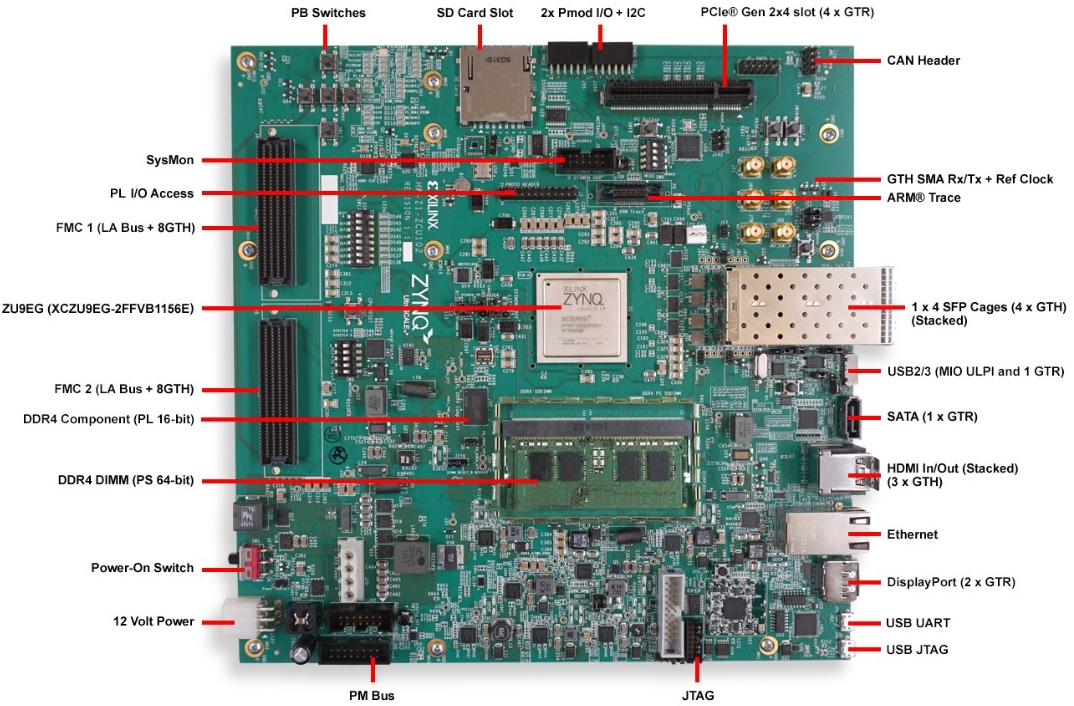
\includegraphics[width=\textwidth]{Images/Hardware/ZCU102-board-overview.jpg}
	\decoRule
	\caption[Xilinx ZCU102 Evaluation Board overview]{Xilinx ZCU102 Evaluation Board overview: \href{https://www.xilinx.com/products/boards-and-kits/ek-u1-zcu102-g.html}{URL}}
	\label{fig:ZCU102-board-overview}
\end{figure}

\subsection{FORTH QFDB}
The Quad-FPGA Daughter Board (QFDB) (Figure \ref{fig:forth-qfdb-daughterboard}) \cite{Implementation-and-Impact-of-an-Ultra-Compact-Multi-FPGA-Board-for-Large-System-Prototyping}, developed by the Foundation of Research and Technology Hellas (FORTH) \cite{FORTH}, combines four of the aforementioned MPSoCs, interconnected with each other. It is a complete platform as well, which provides 16GB of DDR4 memory and an M.2 Solid State Drive (SSD), and some peripherals and interfaces such as Ethernet, JTAG, and UART.

It is designed to be used in servers, with other QFDBs running in parallel, creating a network of FPGAs. The QFDB enables massive hardware designs to be split and deployed into multiple FPGA devices or even multiple QFDB boards. It also enables the deployment of hardware designs into a high number of FPGAs for increased parallelism.

\section{Characteristics}

\begin{table}[H]
	\caption{Scale and bit-width of input and activations}
	\label{tab:scale-and-bit-width-of-input-and-activations}
	\centering
	\begin{tabular}{llll}
		\toprule
		\textbf{Layer} & \textbf{Scale} & \textbf{Theoretical bit-width} & \textbf{Practical bit-width}\\
		\midrule
			Input & 7 & 8 & 8\\
			Conv1 & 5 & $16 + \lceil \log_2 3 * 11 * 11 \rceil = 25 $ & 17\\
			Conv2 & 5 & $16 + \lceil \log_2 64 * 5 * 5 \rceil = 27$ & 14\\
			Conv3 & 5 & $16 + \lceil \log_2 192 * 3 * 3 \rceil = 27$ & 15\\
			Conv4 & 6 & $16 + \lceil \log_2 384 * 3 * 3 \rceil = 28$ & 15\\
			Conv5 & 5 & $16 + \lceil \log_2 256 * 3 * 3 \rceil = 28$ & 17\\
			FC1 & 5 & $16 + \lceil \log_2 9216 \rceil = 30$ & 17\\
			FC2 & 6 & $16 + \lceil \log_2 4096 \rceil = 28$ & 17\\
			FC3 & 6 & $16 + \lceil \log_2 4096 \rceil = 28$ & 17\\
		\bottomrule\\
	\end{tabular}
\end{table}

\section{Scheduling}

\begin{figure} [H]
	\centering
	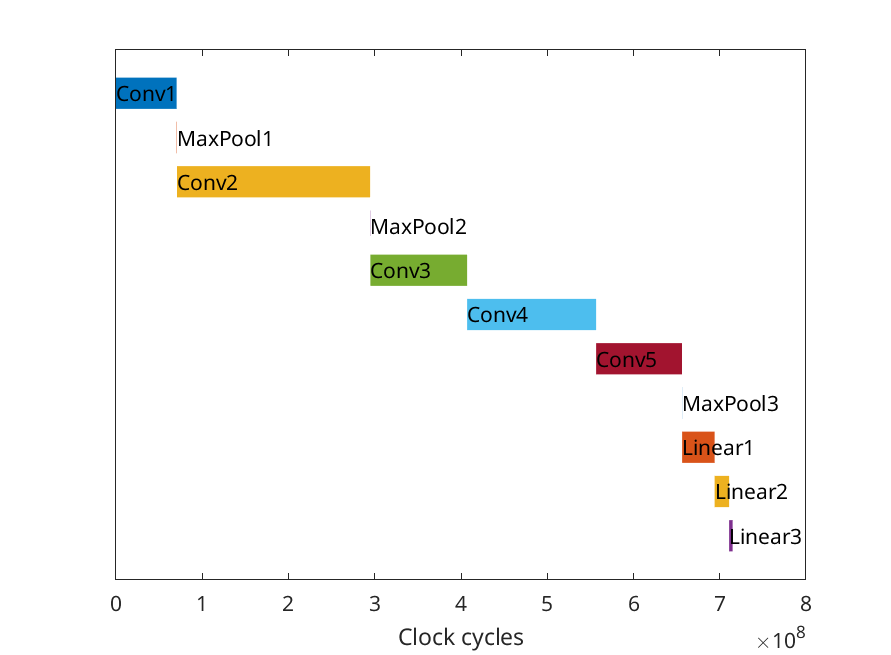
\includegraphics[width=\textwidth]{Images/Scheduling/Serial.png}
	\decoRule
	\caption[AlexNet serial execution]{AlexNet serial execution: Convolution layers consume 90\% of total clock cycles needed for a full inference.}
	\label{fig:ZCU102-board-overview}
\end{figure}
